\section{Efectuarea lucrarii de laborator}



\subsection{Tasks and Points}



Basic Level (nota 5 $||$ 6) : 

-Realizeaza un mini site cu 3 pagini statice


Normal Level (nota 7 $||$ 8):

-Site-ul trebuie sa pastreze toata informatia intr-o baza de date


Advanced Level (nota 9 $||$ 10):

-Site-ul trebuie sa contina AJAX Requests.

-Implimentarea XHR sau JSON responses. Unele informatii trebuie sa fie dinamic incarcata pe pagina

\subsection{Analiza lucrarii de laborator}


Linkul la repozitoriu: \texttt{https://github.com/dumitritag/MIDPS-lab}


Dezvoltarea de aplicatii web presupune doua provocari tehnice distincte: partea grafica, care imbraca intr-un mod ergonomic aplicatia (webdesign), si dezvoltarea propriu-zisa a motorului aplicatiei (dezvoltarea web).

Lucrarea data de laborator consta in crearea unui website pentru a acumula cunostinte mai profunde in Web Development. IDE ales de mine este NetBeans 8.2, iar limbajul de programare este php, HTML/CSS. Am lucrat cu bazele de date MySQL, serverul local WAMP si am operat cu Request-urile AJAX. 

Tematica website-lui meu este top tipurile de cafea. Este compus din 5 pagini: Casa, Cafea, Magazine, Despre si Management. Pagina Casa contine informatie generala despre cafea, efecte negative, efecte pozitive. Pagina Cafea contine tipurile de cafea si descrierea lor, informatia fiind stocata in baza de data phpMySQL. Pagina Magazine contine informatii despre unde se pot gasi aceste tipuri de cafea, adresa , poza lor. In pagina Management am implimentat CMS (Content Management System) prin adaugarea unui nou tip de cafea, incarcarea unei imagini. 

Un sistem de administrare a continutului sau CMS este un sistem software creat pentru automatizarea cit mai deplina a gestiunii continutului, in special a site-urilor web. Scopul este de a reduce sau elimina interventia programatorilor la editarea si administrarea site-urilor lor.


Am intilnit probleme cu operatiile cu implementarea Ajax requests .  
 



\subsection{Imagini}




\begin{figure}[!ht]
	
	\centering
	
	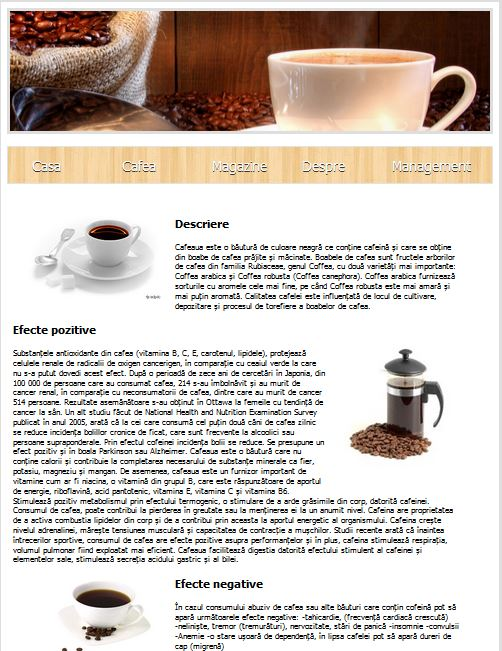
\includegraphics[width=0.5\textwidth]{Cattura.JPG}
	
	\caption{Pagina Casa}
	
	\label{Im_label}
	
\end{figure}

\begin{figure}[!ht]
	
	\centering
	
	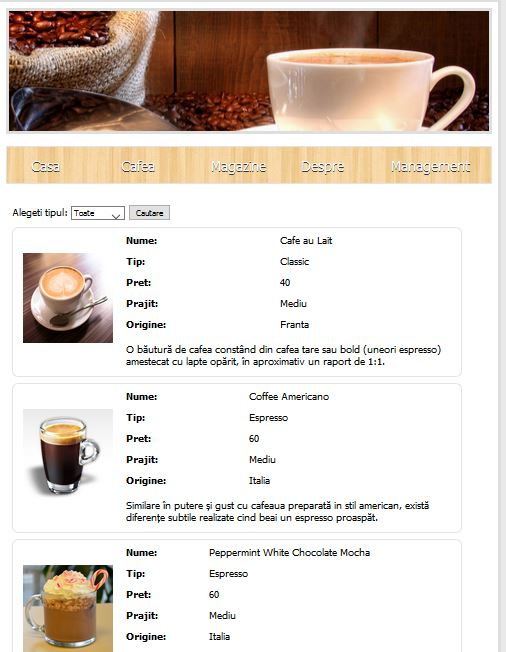
\includegraphics[width=1.0\textwidth]{Cattura1.JPG}
	
	\caption{Pagina Cafea}
	
	\label{Im_label}
	
\end{figure}

\begin{figure}[!ht]
	
	\centering
	
	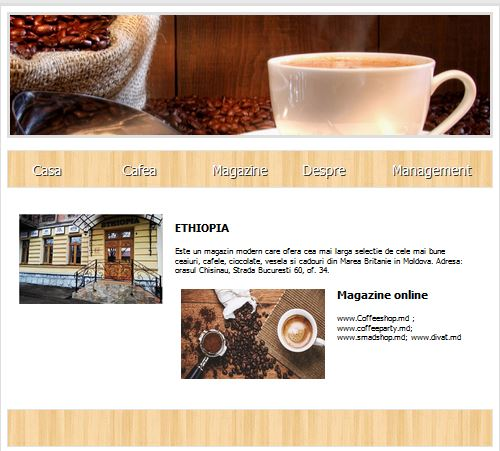
\includegraphics[width=1.0\textwidth]{Cattura2.JPG}
	
	\caption{Pagina Magazine}
	
	\label{Im_label}
	
\end{figure}

\begin{figure}[!ht]
	
	\centering
	
	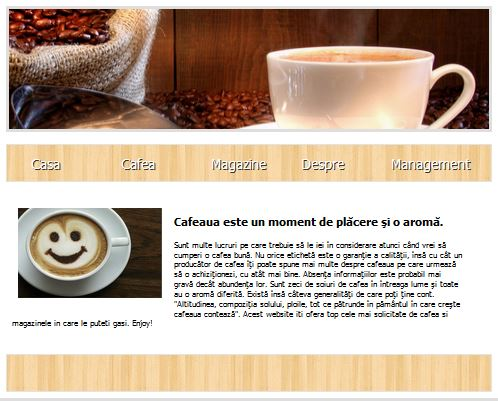
\includegraphics[width=1.0\textwidth]{Cattura3.JPG}
	
	\caption{Pagina Despre}
	
	\label{Im_label}
	
\end{figure}

\begin{figure}[!ht]
	
	\centering
	
	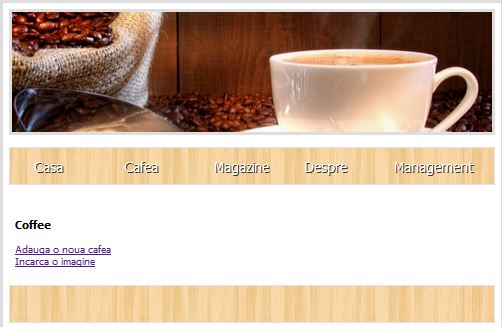
\includegraphics[width=1.0\textwidth]{Cattura4.JPG}
	
	\caption{Pagina Management}
	
	\label{Im_label}
	
\end{figure}


\begin{figure}[!ht]
	
	\centering
	
	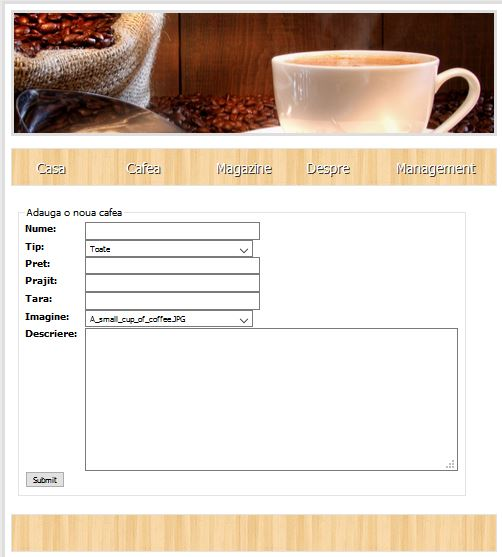
\includegraphics[width=1.0\textwidth]{Cattura5.JPG}
	
	\caption{Adaugarea unui tip de cafea}
	
	\label{Im_label}
	
\end{figure}

\begin{figure}[!ht]
	
	\centering
	
	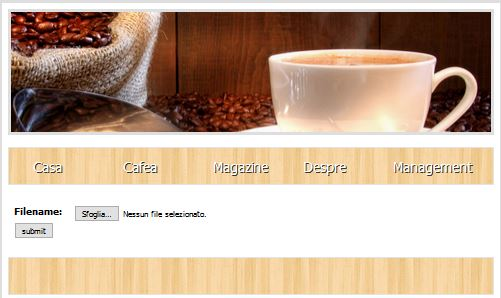
\includegraphics[width=1.0\textwidth]{Cattura6.JPG}
	
	\caption{Adaugarea unei imagini}
	
	\label{Im_label}
	
\end{figure}

\begin{figure}[!ht]
	
	\centering
	
	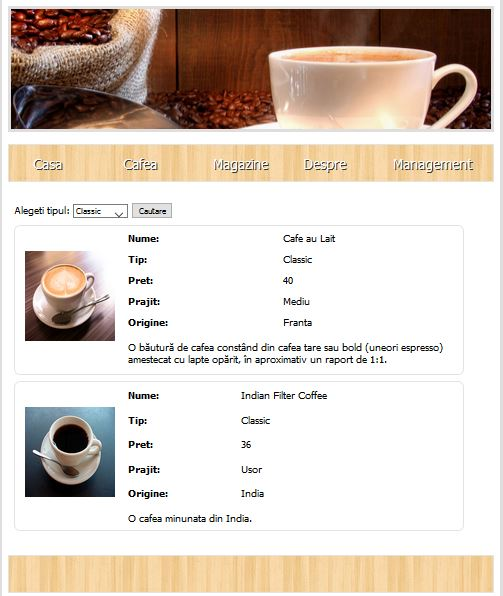
\includegraphics[width=1.0\textwidth]{Cattura7.JPG}
	
	\caption{Ajax}
	
	\label{Im_label}
	
\end{figure}

\clearpage